%
% $Id: cruisespec.tex,v 1.3 2001/08/19 17:09:35 klauko70 Exp $
%
\documentclass[german,12pt,a4paper,oneside]{scrbook}
\usepackage{babel,isolatin1,epsfig,psfig,tabularx,times,fancyheadings,relsize}
\pagestyle{plain}


\title{\center{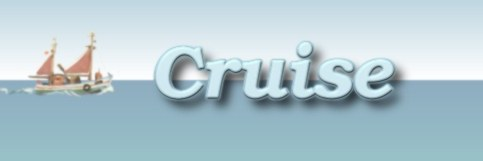
\includegraphics[scale=0.5]{cruise_logo.eps}}\\}
\author{Wolfgang Schrempp \& Klaus Konzept \\	
        \small{http://cruise.berlios.de}
       }


\begin{document}

%%%%%%%%%%%% eigene Kommandos %%%%%%%%%%%%%%%%%%%%%%%%%%%%%%%%%%%%%%

% !!! don�t use \cruise inside \chapter, \section, ... !!!
\newcommand*{\cruise}{\itshape\bfseries\larger\larger C%
        \smaller\smaller\smaller\smaller%
        \hspace{-0.6em}\raisebox{0.3ex}{r}\raisebox{0.65ex}{u}%
        \raisebox{0.4ex}{i}\raisebox{0.15ex}{s}e\larger%
        \larger\normalfont} 


%% klauko70 -> define a new environment for source code 


%%%%%%%%%%%%%%%%%%%%%%%%%%%%%%%%%%%%%%%%%%%%%%%%%%%%%%%%%%%%%%%%%%%%


\maketitle

\newpage

{\LARGE Widmung}
\newline

F�r ..... 

\newpage


\tableofcontents
%\listoffigures
%\listoftables
%\newpage
%%%%%%%%%%%%%%%%%%%%%%%%%%%%%%%%%%%%%%%%%%%%%%%%%%%%%%%%%%%%%%%%%%%%

\pagenumbering{arabic}


%%%%%%%%%%%% Kapitel 1 %%%%%%%%%%%%%%%%%%%%%%%%%
%
% $Id: intro.tex,v 1.2 2001/08/11 17:37:10 klauko70 Exp $
%
\chapter{Einleitung}





%%%%%%%%%%%% Kapitel 2 %%%%%%%%%%%%%%%%%%%%%%%%%
%
% $Id: definitions.tex,v 1.3 2001/08/19 17:09:35 klauko70 Exp $
%
\chapter{Definitionen}

\section{Cruise}
Comfortable Remark Based User Interface for Source Editing

\section{Interpretation}
Die Interpretation ist die Abarbeitung der einzelnen \cruise-Zeilen. Diese findet je Sourcefile genau einmal statt und zwar unmittelbar nach dem Start von \cruise.

\section{Interaktion}
Die Interaktion ist die Einwirkung mit Hilfe von Mauszeiger und/oder Tastatur, auf das mit dem \cruise-Interpreter erzeugte Benutzerinterface.

\section{Ersteller}
Der Ersteller ist diejenige Person, die in ein Sourcefile \cruise-Zeilen einf�gt.

\section{Benutzer}
Der Benutzer ist diejenige Person, die mit dem erzeugten Benutzerinterface interagiert.

\section{Sourcefile}
Das Sourcefile ist die Datei, in die der Ersteller \cruise-Zeilen einf�gt, um eine
\cruise-Funktionalit�t zu erreichen. Ein Sourcefile kann beispielsweise ein
bash-Script, ein Assmbler-Code, ein C-Source-Code oder ein Tex-File sein.

\section{Cruise-Zeile}
Eine \cruise-Zeile wird in das Sourcefile eingef�gt. Damit der Zielprozess die
\cruise-Zeile unbeachtet l��t, mu� die \cruise-Zeile als Kommentar in das Sourcefile eingef�gt werden. Die Einleitung dieses Kommentars richtet sich nach Art des
Zielprozess'

\section{Zielprozess}
Der Zielprozess ist das Programm f�r den das Sourcefile eigentlich gedacht ist.

\section{Ausgabe}
Die Ausgabe ist die Datei, die nach Interpretation des Sourcefiles und anschliessender Interaktion durch den Benutzer von \cruise\ erzeugt wird.


%% klauko70 -> a nice chart would help to understand the above









%%%%%%%%%%%% Kapitel 3 %%%%%%%%%%%%%%%%%%%%%%%%%
%
% $Id: features.tex,v 1.3 2002/02/12 22:15:32 wolli Exp $
%
\chapter{Eigenschaften}
\section{Offenheit}
\cruise ist so entwickelt, dass es sich leicht erweitern l�sst. Die
Schnittstellen nach au�en sind standardisiert, so dass sich \cruise leicht in
eine vorhanden Umgebung einbauen l�sst.

Das Konzept von \cruise erlaubt es das Werkzeug f�r spezielle Probleml�sungen
anzupassen und zu erweitern.

\section{Einfache Benutzbarkeit}
Die Standarteinstellungen von \cruise sind so, dass Standartprobleme mit einem
minimalen Aufwand gel�st werden k�nnen. Nicht desto trotz lassen sich durch die
Offenheit auch komplexe Probleme l�sen.


%%%%%%%%%%%% Kapitel 4 %%%%%%%%%%%%%%%%%%%%%%%%%
%
% $Id: commands.tex,v 1.5 2002/03/24 01:03:38 wolli Exp $
%
\chapter{Cruise-Kommandos}
\section{Optionen}

\subsection{Source Referenz}

Jede Referenzangabe wird durch eine Referenz-Typ-Angabe eingeleitet. 
Die Typ-Angabe wird in Form einer Option dem Cruise-Kommando mitgeteilt. 


\begin{description}
\item[Dateiname:]
\begin{tabbing}
\hspace{10em}\=\\
Syntax:		\>-f\am{filename}\\
default-Wert:	\>aktuelle Datei\\
Beispiel:	\>\verb#-f ~/.bashrc#\\
		\>\verb#-f /usr/local/share/readme.txt#\\
\end{tabbing}
Mit dieser Option wird wird auf eine bestimmte Datei verwiesen. Existiert diese Datei nicht, so wird eine Fehlermeldung
ausgegeben.

\item[Zeile:]
\begin{tabbing}
\hspace{10em}\=\\
Syntax:		\>-l \am{absolute\_line}\\
		\>-l +\am{relative\_line}\\
		\>-l -\am{relative\_line}\\
default-Wert:	\>-l +1	(n�chste Zeile)\\
Beispiel:	\>\verb#-l 4  #(Zeile 4)\\
		\>\verb#-l +2 #(die �bern�chste Zeile)\\
		\>\verb#-l -1 #(die vorige Zeile)\\
\end{tabbing}
Mit dieser Option wird auf eine Zeile verwiesen. Ist die referenzierte Zeilennummer gr��er, als die Anzahl der Zeilen in
der referenzierten Datei so wird auf die letzte Zeile verwiesen. Ist die referenzierte Zeilennummer negativ, so wird auf
die erste Zeile der Datei verwiesen.


\item[Spalte:]
\begin{tabbing}
\hspace{10em}\=\\
Syntax:		\>-c  \am{absolute\_column}\\
		\>-c \#\am{field}\\
default-Wert:	\>-c \#1  (erstes Feld)\\
Beispiel:	\>\verb#-c 3  #(dritte Spalte)\\
		\>\verb+-c #4 +(viertes Feld)\\
\end{tabbing}
Mit dieser Option wird auf eine Spalte verwiesen. Ist die referenzierte Spaltennummer gr��er, als die Anzahl der Spalten in
der referenzierten Zeile so wird auf die letzte Spalte verwiesen. Ist die referenzierte Spaltennummer negativ, so wird auf
die erste Spalte der Zeile verwiesen.

	
\item[Spaltentrenner:]
\begin{tabbing}
\hspace{10em}\=\\
Syntax:		\>-cd \am{column\_delimiter}\\
default-Wert:	\>-cd ws  (whitespace: Tabulator und Leerzeichen)\\
Beispiel:	\>\verb#-cd ","  #(Komma)\\
		\>\verb#-cd " "  #(ein Leerzeichen)\\
\end{tabbing}


Idee: Regul�rer Ausdruck als Spaltentrennerdefinition !


\item[Marke:]
\begin{tabbing}
\hspace{10em}\=\\
Syntax:		\>-m \am{mark}\\
default-Wert:	\>-  (kein default-Wert)\\
Beispiel:	\>\verb#-m mark_1#\\
\end{tabbing}


\item[URL:]
\begin{tabbing}
\hspace{10em}\=\\
Syntax:		\>-u \am{url}\\
default-Wert:	\>-  (kein default-Wert)\\
Beispiel:	\>\verb#-u ftp://ftp.suse.de/misc/readme.txt#\\
\end{tabbing}

\item[Zeiger oben:]
\begin{tabbing}
\hspace{10em}\=\\
Syntax:		\>\^{ }\\
default-Wert:	\>-  (kein default-Wert)\\
Beispiel:	\>\verb#^#\\
\end{tabbing}


\item[Zeiger unten:]
\begin{tabbing}
\hspace{10em}\=\\
Syntax:		\>v\\
default-Wert:	\>-  (kein default-Wert)\\
Beispiel:	\>\verb#v#\\
\end{tabbing}

\end{description}

	
\subsubsection{Anwendungs-Beispiel 1}

Annahme: das cruise Token w�re "\$c\$".
Mit folgendem Beispiel wird auf die Zahl hinter 'MAX\_NUM' referenziert.

\begin{verbatim}
$c$ menubutton -c #3 -ol {110 220 214 889}
#define MAX_NUM 214
\end{verbatim}
\begin{itemize}
\item -c \#3 verweist auf das dritte Feld
\item Dateiname wurde nicht angegeben, also aktuelle Datei
\item Zeile wurde nicht angegeben, also n�chste Zeile
\item Spaltentrenner wurde nicht angegeben, also whitespace
\end{itemize}

\subsubsection{Anwendungs-Beispiel 2}

Annahme: das cruise Token w�re "\$c\$".
Mit folgendem Beispiel wird auf die Zahl hinter dem 
Gleicheitszeichen referenziert.


\begin{verbatim}
$c$ menubutton -c #4 -l +2 -ol {3.14 3.141 3.1415 3.14159} 
// declaration and definition of PI
double pi = 3.1415 ;
\end{verbatim}
\begin{itemize}
\item -c \#4 verweist auf das vierte Feld
\item -l +2 verweist auf die �bern�chste Zeile
\end{itemize}


\subsection{Textoptionen}

Mit einer Textoption werden Textinformationen f�r den Benutzer an das jeweilige Kommando �bergeben.

\begin{description}
\item[Beschriftung:]
\begin{tabbing}
\hspace{10em}\=\\
Syntax:		\>-t\am{text}\\
default-Wert:	\>-\\
Beispiel:	\>\verb#-t "Neuer Wert:"#\\

\end{tabbing}
Der mit der Option angegebene Text wird zur Beschriftung des Bedienelementes verwendet.

\item[Hilfetext:]
\begin{tabbing}
\hspace{10em}\=\\
Syntax:		\>-h\am{text}\\
default-Wert:	\>-\\
Beispiel:	\>\verb#-h "W�hlen sie einen Wert zwischen 0 und 255 !"#\\
		\>\verb#-h $HELPTEXT#\\
\end{tabbing}
Wird mit einem Kommando ein Bedienelement mit Hilfeknopf erzeugt, so wird mit diesem Kommando der Text �bergeben, der im Textfenster des Hilfeknopfs erscheinen soll.


\item[Parameterliste:]
\begin{tabbing}
\hspace{10em}\=\\
Syntax:		\>-ol\am{text1 text2 text3 text4}\\
default-Wert:	\>-\\
Beispiel:	\>\verb#-ol {9600 19200 57200}#\\

\end{tabbing}
Kommandos welche eine Liste von ausw�hlbaren Texten anbieten erhalten mit dieser Option die Auswahlliste.

\end{description}











%
% $Id: cruise_message.tex,v 1.2 2002/02/12 22:15:32 wolli Exp $
%
\section{Kommando 'message'}
\kw{message} \am{String}

\subsection{look and feel}

\includegraphics{cruise_message.eps}
\subsection{Verhalten w�hrend Interpretation}
Erzeugt eine Box mit dem Textinhalt \am{String}.

\subsection{Verhalten bei Interaktion}
Keine Interaktion m�glich

\subsection{Beispiel}

\verb*|message "Noch ein Text"|

erzeugt eine Box mit dem Inhalt: \op{Noch ein Text}.

\verb*|message 41+1=[expr 41 + 1]|

erzeugt eine Box mit dem Inhalt: \op{41+1=42}.















%
% $Id: cruise_listbox.tex,v 1.1 2001/08/03 20:17:16 klauko70 Exp $
%
\section{Kommando 'listbox'}
listbox LIST DEFAULT

\subsection{look and feel}
Das Bild zeigt die Listbox w�hrend der Interaktion.

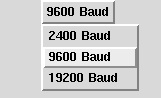
\includegraphics{cruise_listbox.eps}
\subsection{Verhalten w�hrend Interpretation}
Erzeugt eine Box mit dem Inhalt DEFAULT.

\subsection{Verhalten bei Interaktion}
Wird die Box mit dem Inhalt DEFAULT angeklickt, so �ffnet sich eine Auswahlliste
mit den Eintr�gen wie sie in der Liste LIST angegeben wurden. Der Benutzer kann
nun durch Auswahl eines Listeneintrags den neuen Wert bestimmen. Die
Auswahlliste verschwindet und anstelle des DEFAULT Wertes steht der neue
ausgew�hlte Wert.

\subsection{Beispiel}

\verb*|listbox {"2400 Baud" "9600 Baud" "19200 Baud"} "9600 Baud"|

erzeugt bei Interaktion eine Auswahlliste wie oben dargestellt.





%%%%%%%%%%%%%%%%Anhang %%%%%%%%%%%%%
\end{document}





















